\documentclass[aspectratio=169, 13pt]{beamer}
\usepackage[russian, english]{babel}
\usepackage[utf8]{inputenc}

\usepackage{graphicx}
\usepackage{sidecap}
\usepackage{mathtools}
\usepackage{appendixnumberbeamer}
\usepackage{bbm}

\newcommand{\sbrkt}[1]{\left[ #1 \right]}
\DeclarePairedDelimiter\bra{\langle}{\rvert}
\DeclarePairedDelimiter\ket{\lvert}{\rangle}
\DeclarePairedDelimiterX\braket[2]{\langle}{\rangle}{#1 \delimsize\vert #2}
\newcommand{\rbrkt}[1]{\left( #1 \right)}
\newcommand{\lbrkt}[1]{\left< #1 \right>}


\graphicspath{{Pics/}}
%beamer  theme's used to be here :)
\usetheme{mipt_beamer}
\usefonttheme[onlymath]{serif}

\title{CPW resonators\\Noise and Decoherence vs Spin Echo\\Xmon cQED}
\author{Fedorov G. P., Moscow Institute of Physics and Technology}
\date{\today}

\setlength{\jot}{15pt}
\setbeamertemplate{footline}[page number]
\renewcommand*{\inserttotalframenumber}{\insertpresentationendpage}
\newcommand{\Tr}[1]{\text{Tr}\left[#1\right]}

\AtBeginSection[]
{
  \begin{frame}[plain]
    \tableofcontents[currentsection]
    \addtocounter{page}{-1}
  \end{frame}
}



\begin{document}
  
{
\begin{frame}[plain]
  \titlepage
\end{frame}
}

\selectlanguage{russian}

\frame[plain]{\tableofcontents}



\section{Coplanar waveguide resonators}
\subsection{Quality factors and effective parameters}
\begin{frame}[c]\frametitle{\secname}\framesubtitle{\subsecname}

Capacitively coupled CPW resonator as a lumped-element model: 

\vspace{0.5cm}
\begin{columns}[c]
\onslide<1,2,3>{
	\column{0.45\textwidth}
	\centering
	\includegraphics[width=0.9\textwidth]{resonator}

}
\onslide<2,3>{
	\column{0.1\textwidth}
	\centering
	{ \Huge $\Rightarrow$ }
\column{0.45\textwidth}

\includegraphics[width=0.9\textwidth]{resonator_equiv}
}
\end{columns}
\only<1>{
	\vfill
}
\only<2>{
\vspace{0.5cm}
	\[
	R^{*} = \frac{1+\omega^2 C_\kappa^2 (Z_0/2)^2}{\omega^2 C_\kappa^2 (Z_0/2)	}, \quad
	C^{*} = \frac{C_\kappa}{1+\omega^2 C_\kappa^2 (Z_0/2)^2} \approx C_\kappa\ (\text{for our case}). 
	\]
}
\only<3>{
\vspace{0.5cm}
	\[
	Q_i =  \omega (C+C^{*}) R_{in}, \quad
	Q_e = \omega (C+C^{*}) R^{*}, \quad
	Q_l = \omega (C+C^{*})  \frac{1}{1/R^{*}+1/R_{in}}. 
\]
}
\end{frame}

\frame{\frametitle{\secname}\framesubtitle{\subsecname}
Loaded, internal and external quality factors depending on $C_\kappa$:

\centering

\vspace{0.5cm}
\includegraphics[width=\textwidth]{q-factors}
}

\subsection{S-parameters}
\begin{frame}[c]\frametitle{\secname}\framesubtitle{\subsecname}
General algorithm for calculating S-parameters of a given device:

\vspace{0.5cm}
\begin{columns}[c]
\column{0.5\textwidth}
\centering

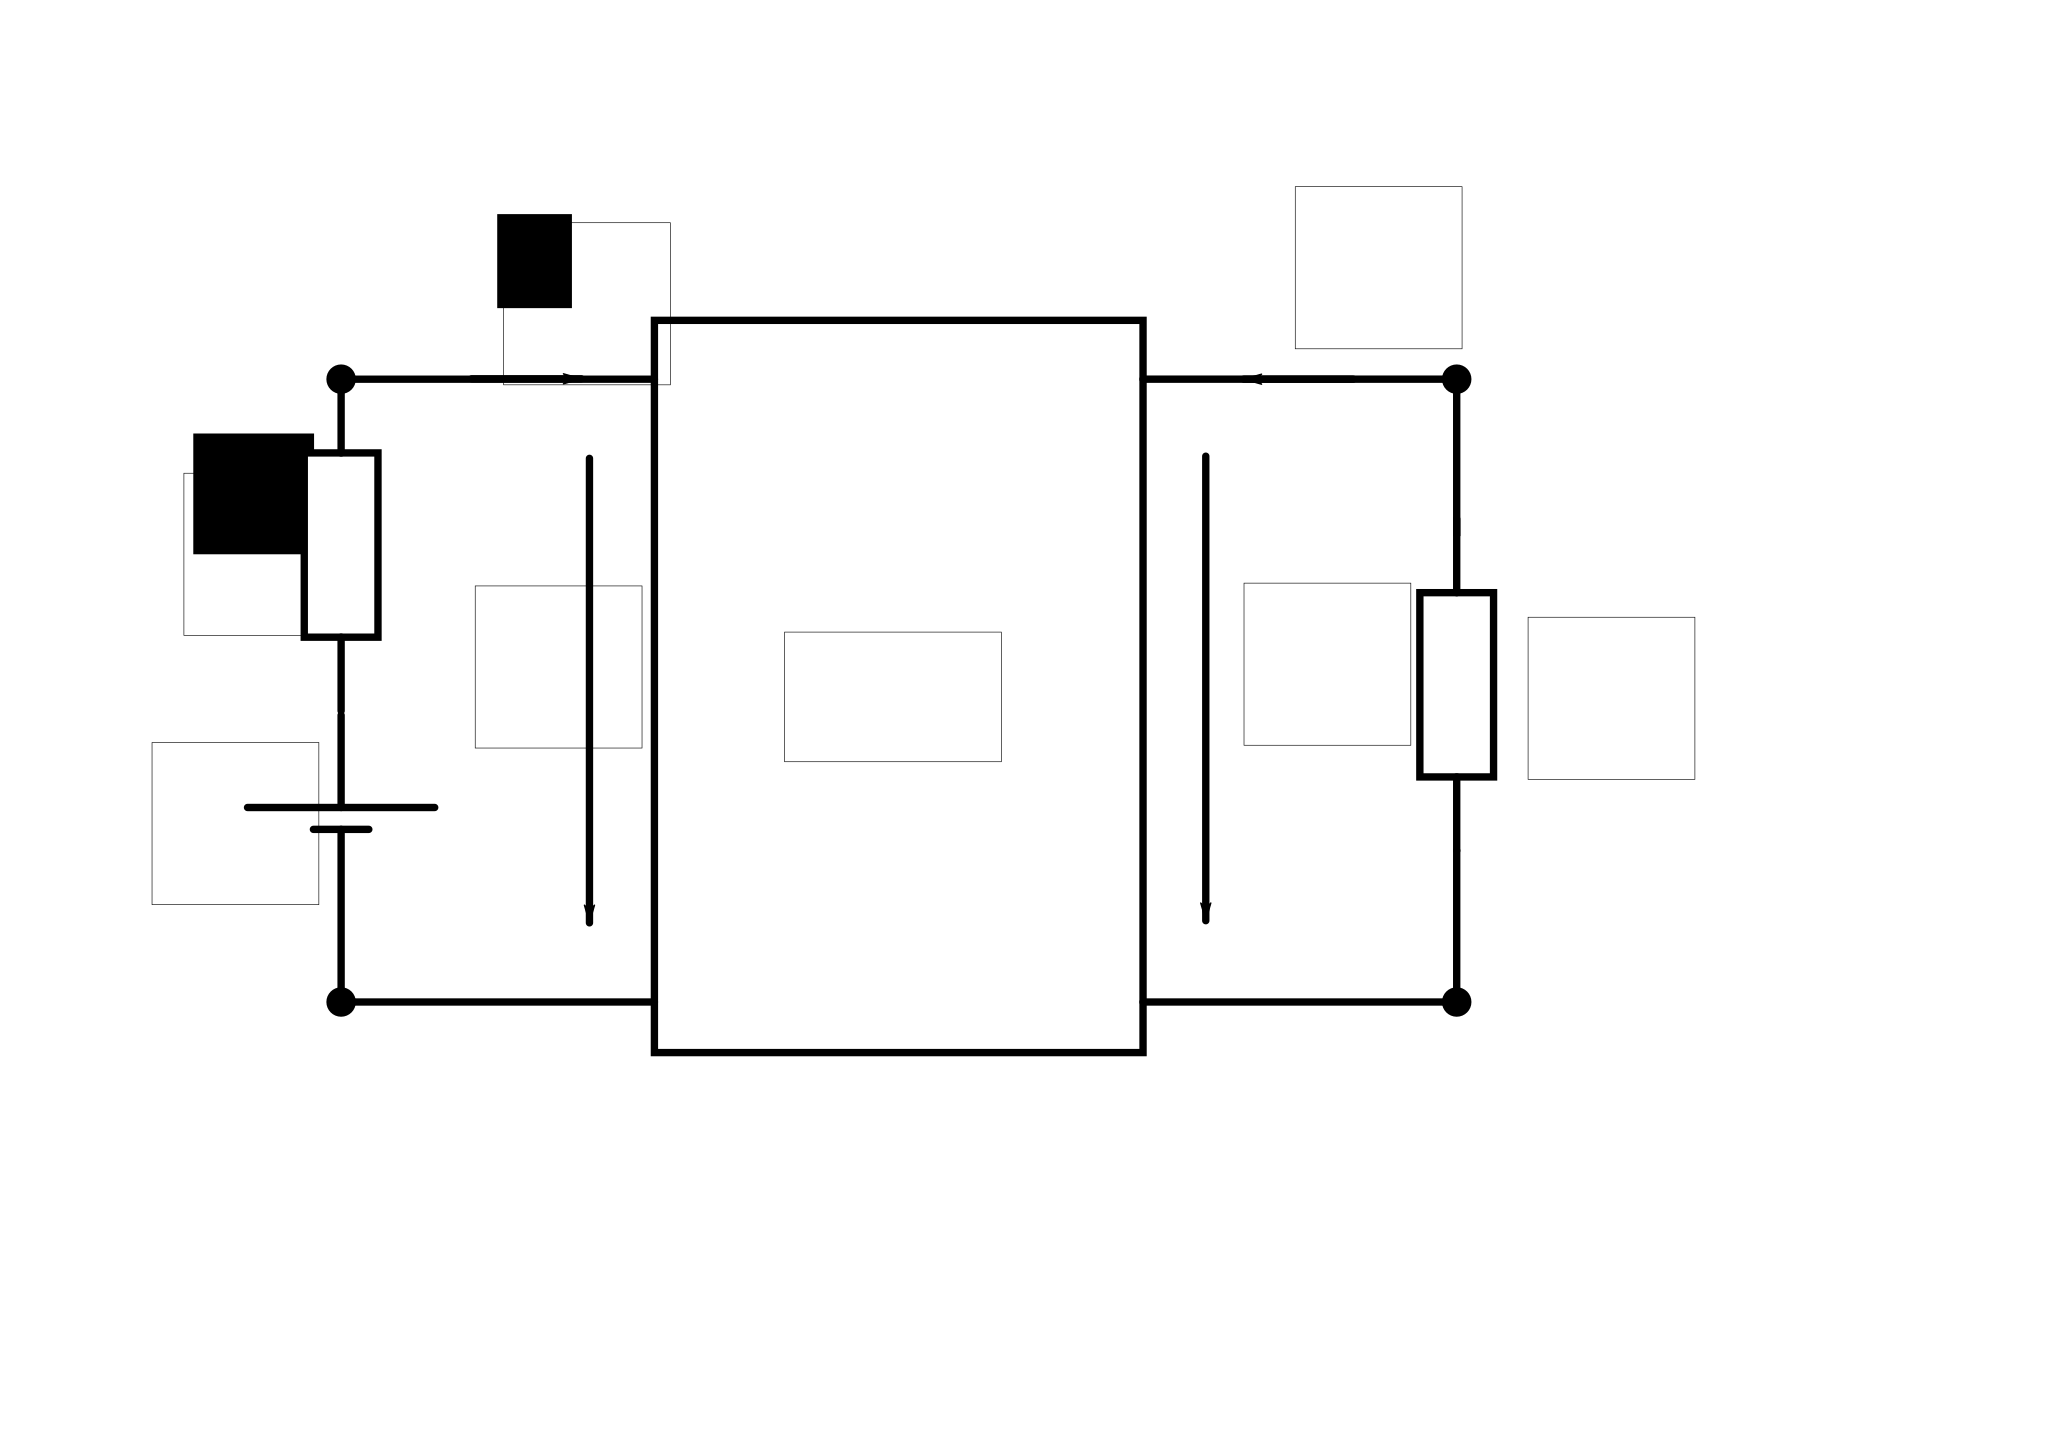
\includegraphics[width=0.95\textwidth]{tl_scheme_general}
\column{0.5\textwidth}
\centering

\vspace{0.35cm}
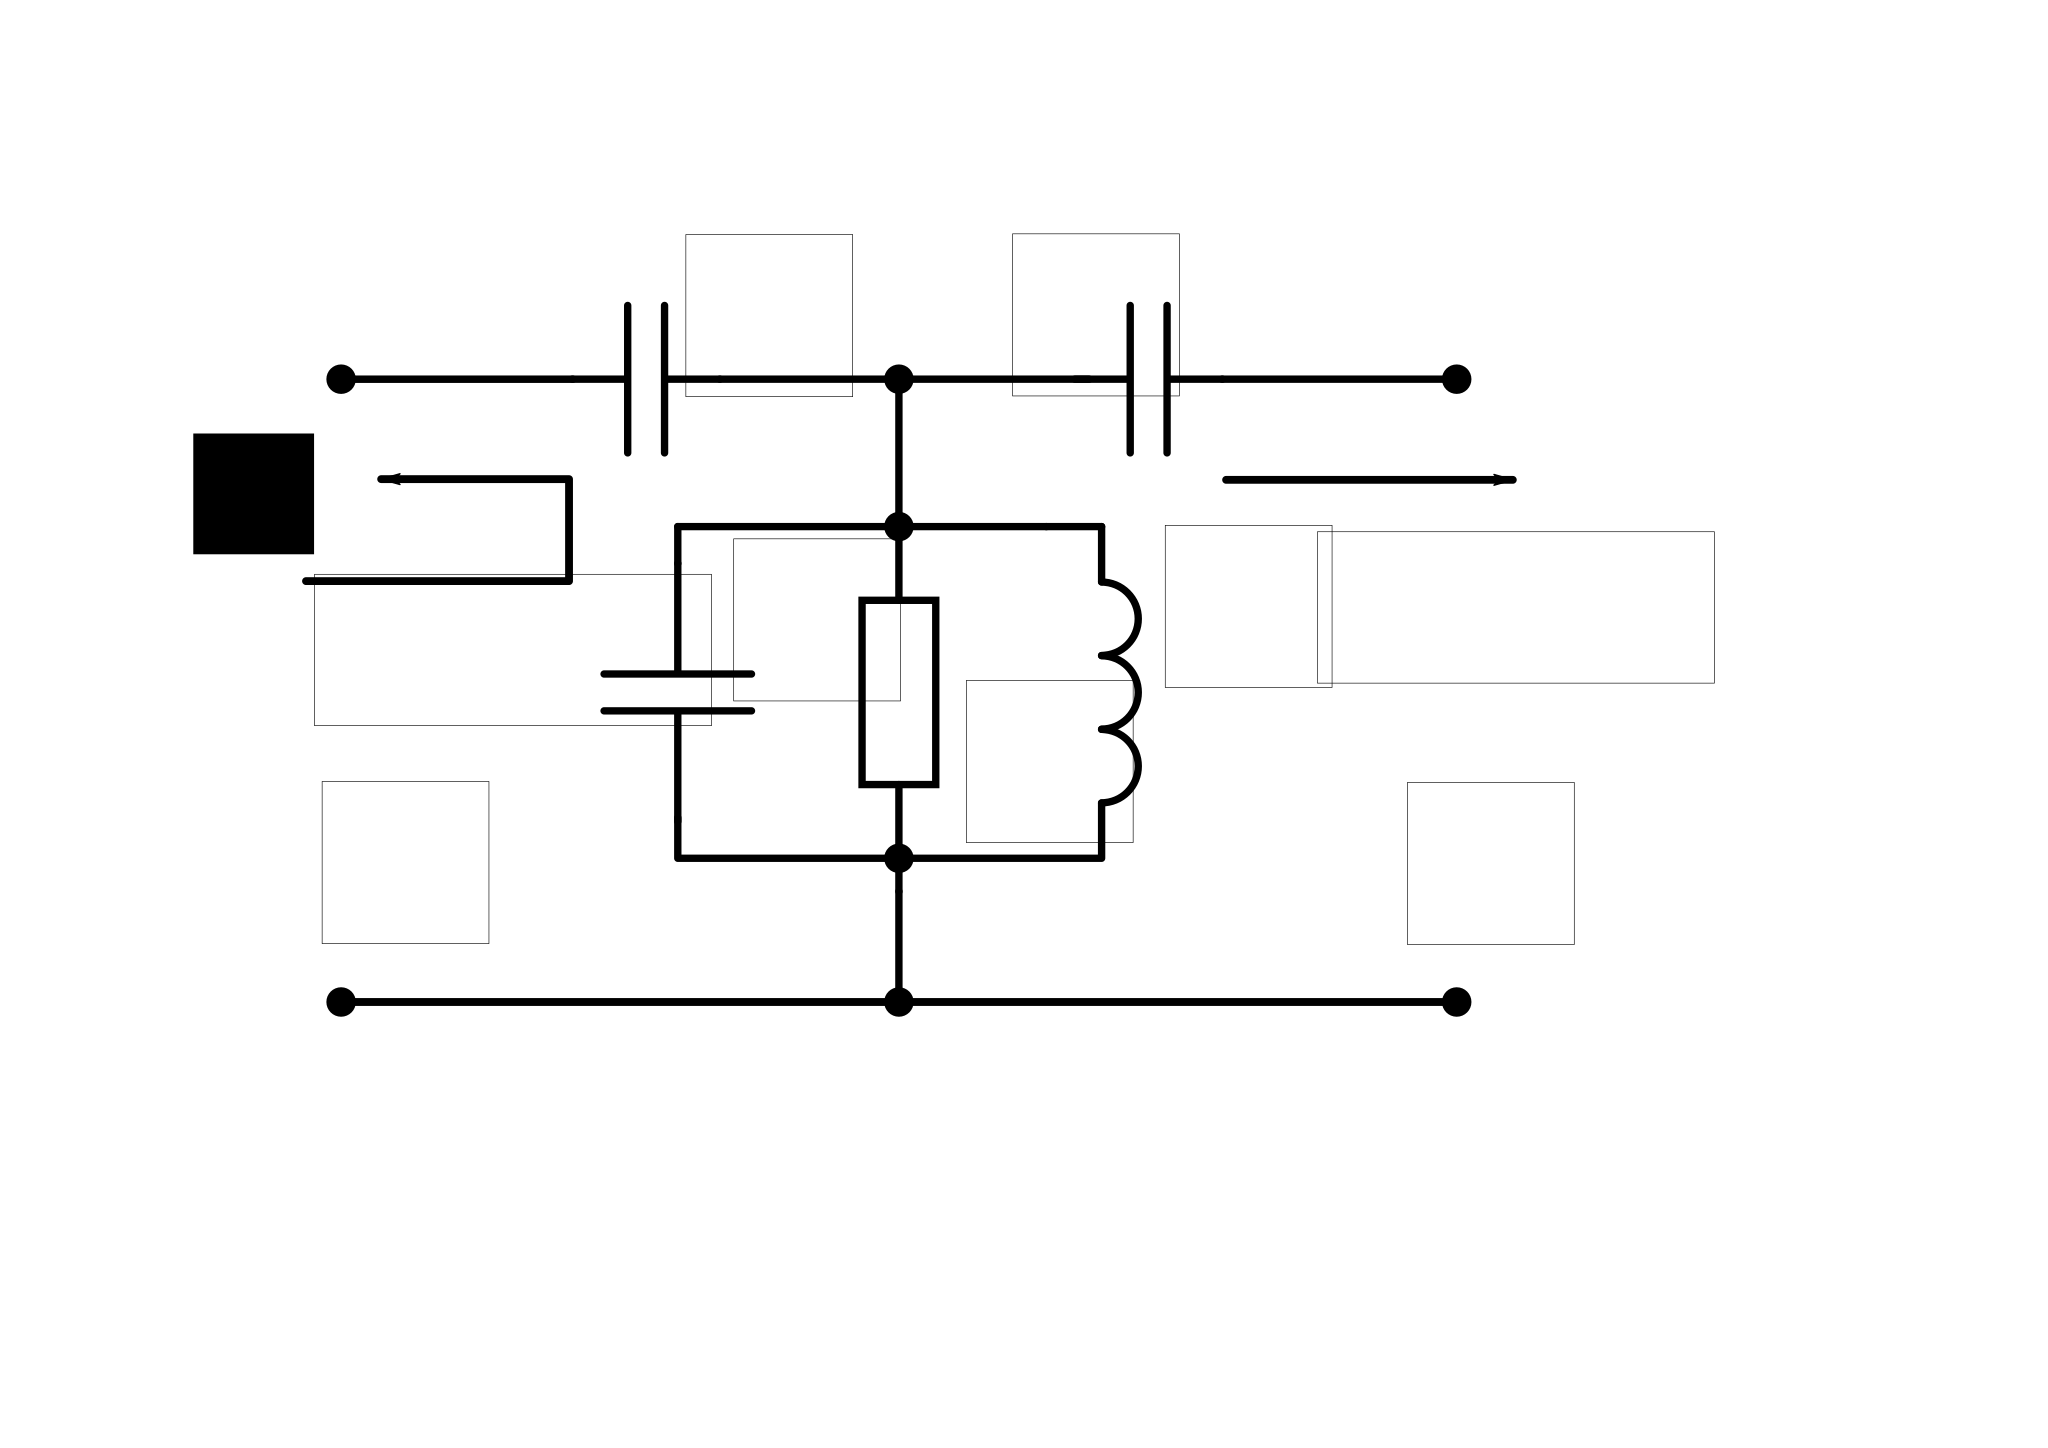
\includegraphics[width=0.8\textwidth]{tl_scheme}
\end{columns}

\begin{equation*}
\text{Kirchgoff's laws}\quad \Rightarrow \quad
\begin{gathered}
V_{1,2} = V_{1,2}^+ + V_{1,2}^- ,\\
I_{1,2} = \frac{ V_{1,2}^+ - V_{1,2}^- }{Z_0}
\end{gathered} \quad \Rightarrow \quad
\rbrkt{\begin{matrix}
V_1^- \\
V_2^-
\end{matrix}} = 
\rbrkt{\begin{matrix}
S_{11} & S_{12} \\
S_{21} & S_{22}
\end{matrix}}
\rbrkt{\begin{matrix}
V_1^+ \\
V_2^+
\end{matrix}}.
\end{equation*}

\end{frame}

\frame{\frametitle{\secname}\framesubtitle{\subsecname}
Transmission spectra for the shunting resonator depending on $C_\kappa$:

\centering
\vspace{0.5cm}
\includegraphics[width=\textwidth]{S21s}
}

\subsection{Xmon design peculiarities}
\begin{frame}[c]\frametitle{\secname}\framesubtitle{\subsecname}
\begin{columns}[c]
\column{0.3\textwidth}
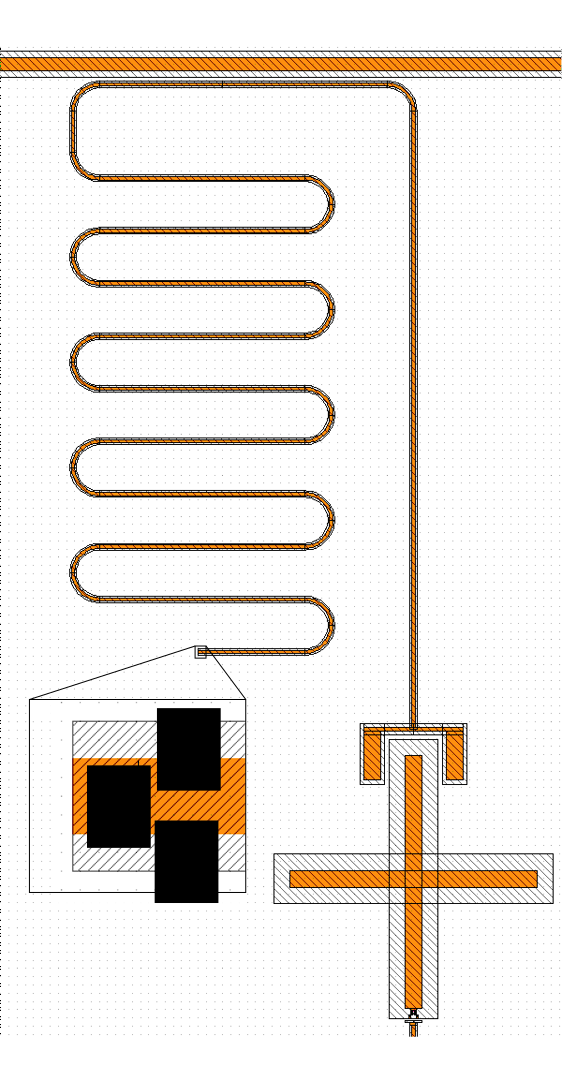
\includegraphics[height=0.9\textheight]{xmonres}
\column{0.7\textwidth}
$l = \lambda/4$ coplanar resonators, $W=4\,\mu m,\ G=2\,\mu m$.

\vspace{0.5cm}
Unconventional coupling area:
 $$C_\kappa^{eff} = C_\kappa \cos \frac{\pi x_\kappa}{2 l}\ ?$$
 $$M_\kappa =\ ?$$
``Claw'' coupler at the open end. Adds up some phase $\phi(\omega)$ and can be replaced by
$$\Delta l = \frac{\phi(\omega_r) c}{2 \omega_r \sqrt{\varepsilon_{eff}}}$$
with extreme accuracy.
\end{columns}
\end{frame}


\subsection{Simulations}
\begin{frame}[c]\frametitle{\secname}\framesubtitle{\subsecname}
\only<1>{
	Resonator without a claw. Frequency expected from the length and $C_\kappa$ (extracted from $Q_L \approx 10^4$) is 7.925 GHz.

	\vspace{0.5cm}
	\begin{columns}[c]
	\column{0.4\textwidth}
	\centering
	\includegraphics[height=0.7\textheight]{xmonres_sim_noclaw}
	\column{0.6\textwidth}
	\centering
	\includegraphics[width=\textwidth]{xmonres_sim_noclaw_res}
	\end{columns}
}
\only<2>{
	Resonator with a claw. Frequency expected from the previous simulation and $\phi$ (also simulated separately for the given claw) is 7.4255 GHz.
	
	\vspace{0.5cm}
	\begin{columns}[c]
	\column{0.4\textwidth}
	\centering
	\includegraphics[height=0.7\textheight]{xmonres_sim_claw}
	\column{0.6\textwidth}
	\centering
	\includegraphics[width=\textwidth]{xmonres_sim_noclaw_res}
	\end{columns}
}

\end{frame}

\section{Noise and decoherence versus Hahn echo technique}
\subsection{Quantum-mechanically treated dephasing}
\frame{\frametitle{\secname}\framesubtitle{\subsecname}

}
\subsection{Classically treated dephasing}
\frame{\frametitle{\secname}\framesubtitle{\subsecname}

}


\subsection{Hahn echo}
\begin{frame}[c]\frametitle{\secname}\framesubtitle{\subsecname}

\end{frame}

\subsection{Noise PSD}
\begin{frame}[c]\frametitle{\secname}\framesubtitle{\subsecname}

\end{frame}

\subsection{Who wins?}
\begin{frame}[c]\frametitle{\secname}\framesubtitle{\subsecname}

\end{frame}

\section{Xmon cQED}


\subsection{Circuit quantization}
\frame{\frametitle{\secname}\framesubtitle{\subsecname}

}

\subsection{Eigenproblem for an isolated Xmon}
\frame{\frametitle{\secname}\framesubtitle{\subsecname}


}

\subsection{Strong driving}
\frame{\frametitle{\secname}\framesubtitle{\subsecname}

}


\subsection{Eigenproblem for a qubit-resonator system}
\frame{\frametitle{\secname}\framesubtitle{\subsecname}

}

\subsection{Dispersive shifts}
\frame{\frametitle{\secname}\framesubtitle{\subsecname} 

}



\appendix


\end{document}